\begin{frame}{$K^0$タグをつけた$"n"$運動量と$n \pi^+ \pi^-$不変質量}
  \begin{tabular}{cc}
    \begin{minipage}{0.5\hsize}
      \footnotesize
      $\pi^+ \pi^-$の不変質量で$K^0$を選んでいる\\
      運動量分布は以下の論文の分布を\\3個のガウス関数で再現\\
      {
        \scriptsize
        Nucl. Phys. A365 (1981), 349
      }
    \end{minipage}
    \begin{minipage}{0.5\hsize}
      \begin{figure}
        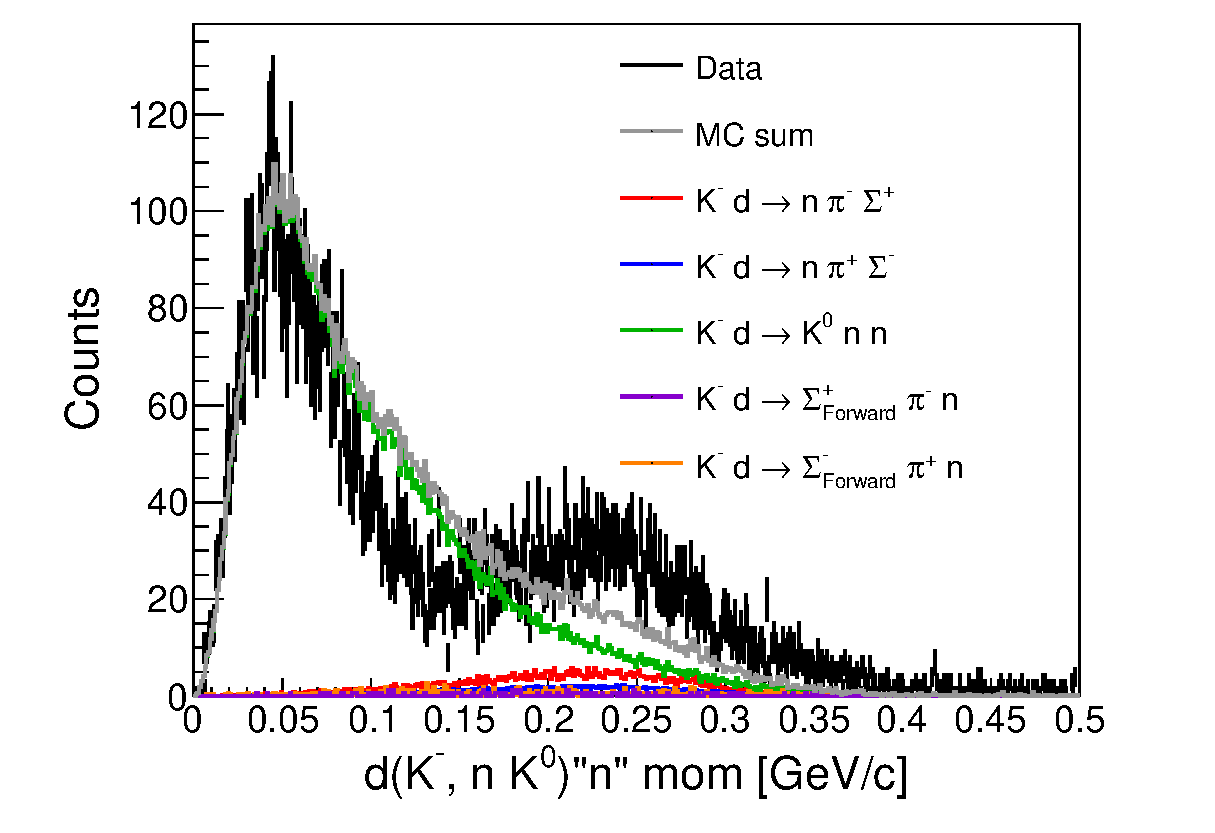
\includegraphics[width=5cm]{../pic/Run78/KN_ana/mmN_mom_K0.eps}
      \end{figure}
    \end{minipage}
  \end{tabular}
  
  \begin{tabular}{cc}
    \begin{minipage}{0.5\hsize}
      \begin{figure}
        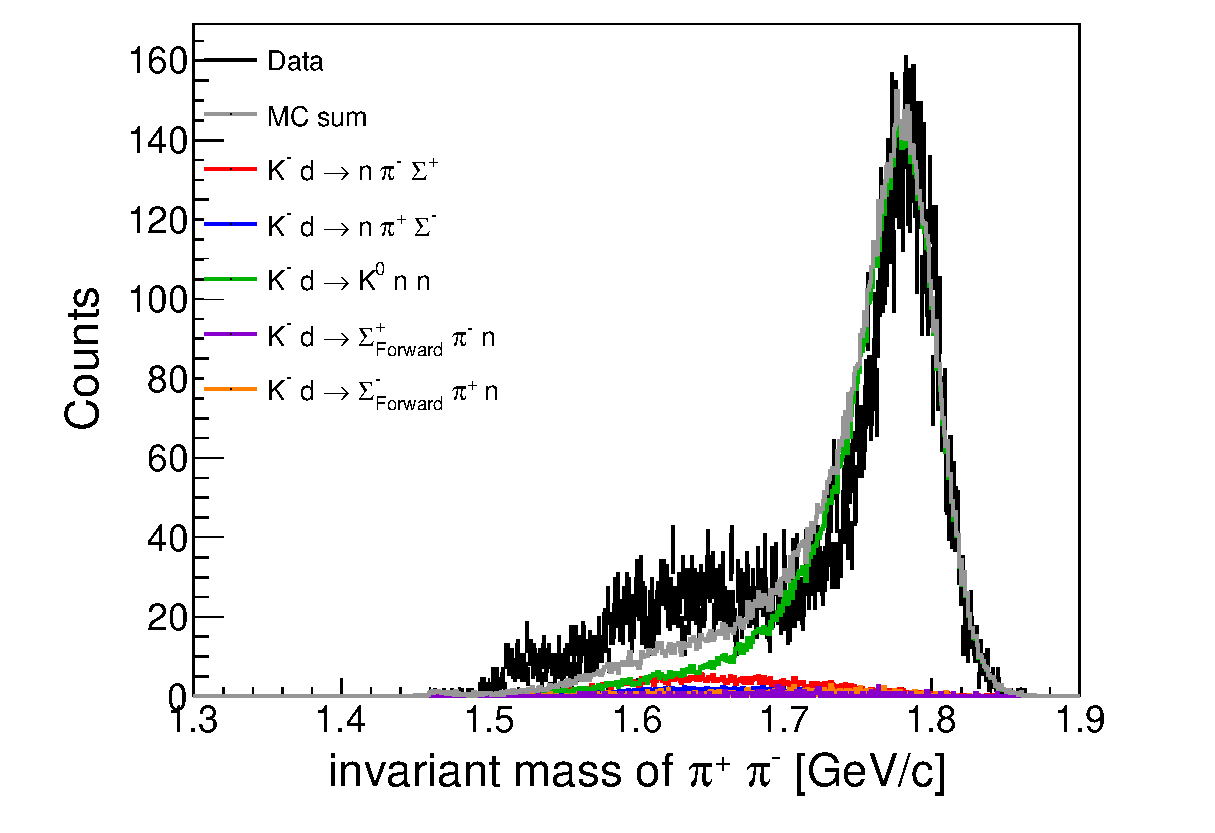
\includegraphics[width=5cm]{../pic/Run78/KN_ana/IM_npipi_K0.eps}
      \end{figure}
    \end{minipage}
    \begin{minipage}{0.5\hsize}
      \begin{figure}
        \includegraphics[width=5cm]{../pic/Run78/KN_ana/mmN_mom_IM_npipi_K0.eps}
      \end{figure}
    \end{minipage}
  \end{tabular}

  $"n"$運動量の高い成分はいる(他の過程からの混入では説明がつかない)
\end{frame}
